\documentclass[a4paper,10pt]{scrarticle}
\usepackage{fontspec}

\usepackage{polyglossia}
\setmainlanguage[variant=british]{english}
\setotherlanguage[babelshorthands=true]{german}

\usepackage{xcolor}
\usepackage{booktabs}
\usepackage{graphicx}
\graphicspath{ {./img/} }
\usepackage{blindtext}
\usepackage{listings}

%\defaultfontfeatures{Scale=MatchLowercase}
\setmainfont[Ligatures=TeX]{Linux Libertine O}
\setsansfont[Ligatures=TeX,Scale=MatchLowercase]{Linux Biolinum O}

\usepackage{typography}

\setlength{\parindent}{0pt}
\reversemarginpar

\newcommand{\loremipsum}{Lorem ipsum dolor sit amet, consectetur adipisici elit, sed eiusmod tempor incidunt ut labore et dolore magna aliqua. Ut enim ad minim veniam, quis nostrud exercitation ullamco laboris nisi ut aliquid ex ea commodi consequat.}

\title{\textnormal{The \textbf{typography} Package}}
\author{Alexander Bernardi}
\date{\today}

\begin{document}
\maketitle

\section{Typography}

The word "typography" in English comes from the Greek roots τύπος [typos ('type')] and -γραφία [-graphia ('writing')].
Typography is the art and technique of arranging type to make written language legible, readable and appealing when displayed.

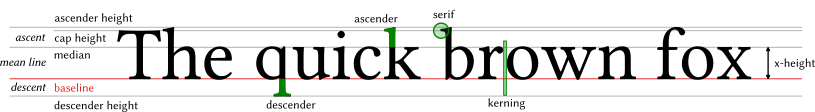
\includegraphics[width=\linewidth]{img/Typography Lines Terms.png} 



\begin{minipage}[t]{0.48\linewidth}
{\fontspec{Latin Modern Roman}\fontsize{10}{12}\loremipsum\\ Latin Modern Roman @ 10pt}
\end{minipage}
\hfill
\begin{minipage}[t]{0.48\linewidth}
{\fontspec{Clarity City}\fontsize{10}{12}\loremipsum\\ Clarity City @ 10pt}
\end{minipage}

\noindent\marginpar{point size} Point size refers to the height of the font but not the height of the letter.
1 point (pt) has been approximated as exactly $\frac{1}{72.27}$ of the inch by Donald Knuth for the default unit of \TeX. A TeX point is 0.351 mm.\par
\medskip
{\centering 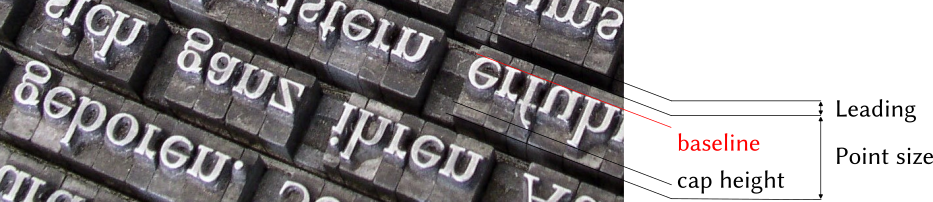
\includegraphics[width=\linewidth]{img/Typography leading.png} \par}
\medskip

\noindent\marginpar{leading} In typography, leading is the space between adjacent lines of type. 
In hand typesetting, leading is the thin strips of lead that were inserted between lines of type in the composing stick to increase the vertical distance between them. 
The thickness of the strip is called leading and is equal to the difference between the size of the type and the distance from one baseline to the next. For instance, given a type size of 10 points and a distance between baselines of 12 points, the leading would be 2 points.\par
\medskip
{\centering 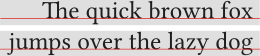
\includegraphics[scale=1]{img/Typography leading font.png} \par}
\medskip

\noindent\marginpar{total height}

\noindent\marginpar{cap height}

\noindent\marginpar{x-height}

\noindent\marginpar{letter-spacing} Letter-spacing adjusts the overall horizontal space between groups of letters.
 
\noindent\marginpar{kerning} Kerning adjusts the horizontal space between specific letter pairs to improve legibility in words that have inconsistent spacing, which makes the text look awkward and unprofessional.

\section{Commands}

\noindent\marginpar{\texttt{getTotalHeight\\setTotalHeight}} Gesamthöhe des fonts
\begin{lstlisting}[language={[AlLaTeX]TeX}]
\getTotalHeight

\newlength\totalheight
\setTotalHeight\totalheight
\the\totalheight

\typo_get_totalheight:n {font parameter}
\typo_set_totalheight:Nn <variable name> <font parameter>
\end{lstlisting}

\noindent\marginpar{\texttt{getCapHeight\\setCapHeight}} Caphöhe des fonts

\section{Lengths}

\noindent\marginpar{charwidth} Durchschnittliche Zeichenlänge der mainfont bei normalsize

\noindent\marginpar{baseline} Optimale Zeilenhöhe der mainfont bei normalsize als baseline

\noindent\marginpar{xheight} Die x-Höhe der mainfont bei normalsize 

\end{document}